\chapter{Conclusiones y Trabajos Futuros}
La estimación de la calidad de imágenes (IQA) es un problema esencial a la hora 
de optimizar el formato y visualización de la información, además es de 
suma importancia para el ámbito biomédico. 
Este TFG aborda la obtención de una métrica de estimación de calidad capaz de evaluar 
representaciones 3D sin referencia, en concreto nubes de puntos, del ámbito biomédico para poder asistir 
en la mejora de los algoritmos de reconstrucción y visualización de dichos objetos. 
La representación común de estas superficies complejas 
suele ser por medio de nubes de puntos~\cite{WhyUsePointCloud}. 
Además, objetos representados en volúmenes de vóxeles o mallas poligonales se pueden 
muestrear en nubes de puntos. Incluso, algunos procesos de adquisición como 
por escaneo o segmentación generan información geométrica en forma de puntos. 
Estos puntos se usan para diversas aplicaciones, 
como medición morfológica, extracción de líneas centrales, 
particionamiento de superficies, registro de formas de tumores o huesos~\cite{WhyUsePointCloud}.
Por todo ello, las contribuciones relativas al IQA en el 
ámbito biomédico son claramente bienvenidas.

En primer lugar, se realizó un estudio de la literatura relativa a la estimación de calidad 
de imágenes 2D, desde los métodos basados en extracción de características de escenas naturales y modelos de ML, 
hasta la extracción automática con DL. 
A continuación, se estudió el uso de estos y otros métodos sobre imágenes médicas 2D.
Posteriormente se analizó el estado del arte de métodos dedicados a representaciones tridimensionales. 
Se observa un salto en complejidad teórica y computacional al tratarse de problemas 
en tres dimensiones. 
Por último, se concluye que no existe hasta el momento 
otra investigación que haya tomado el enfoque novedoso de estimar la calidad de 
reconstrucciones biomédicas 3D. 

Se implementó los métodos del estado del arte de estimación de calidad de objetos 
3D, tanto desde la perspectiva de métodos tradicionales (ML, en donde la extracción 
de características y la clasificación son etapas independientes) como de métodos 
\emph{end-to-end} DL. El primero hace uso de características 
extraídas manualmente utilizando conocimiento humano sobre el sistema visual humano (HVS), 
como fenómenos de planaridad, esfericidad, anisotropía, curvatura, linealidad y consistencia de 
colores de las nubes de puntos, que luego se utilizan para estimar una regresión por 
SVM. En comparativa, de los modelos DL se utilizó un modelo capaz de extraer 
información estática y dinámica de nubes de puntos haciendo uso de múltiples 
proyecciones 2D y de un vídeo del objeto 3D rotando. De esta forma, podemos  
simular el HVS. Para ambos modelos se proponen ajustes y pequeñas mejoras basadas 
en recientes publicaciones y se comparan los resultados. 
Al igual que la tendencia del estado del arte, sale exitoso el modelo DL. 

Para la validación sobre un conjunto de datos médicos se necesitó el desarrollo 
de un conjunto de datos sintético debido a la no existencia de un conjunto de 
datos públicos para este análisis. Para ello se estudiaron y se fabricaron las distorsiones más 
comunes del ámbito biomédico con respecto a las representaciones 3D. Para las etiquetas, 
se hizo uso de las métricas estándar del problema con referencia, que es el subproblema 
más avanzado y que en diversas publicaciones se demuestra la alta correlación 
de esas métricas y el HVS, pudiendo así justificarse el uso de esas 
etiquetas generadas antes que la ejecución de un experimento de estimación 
manual para la obtención de dicha etiqueta según los estándares, experimento que se 
sale del marco temporal y planificación de este proyecto. Se generaron 
un total de 385 representaciones médicas 3D distorsionadas, 11 nubes de puntos 
base, 5 distorsiones a 7 niveles cada una. En las distorsiones se simula 
tanto errores de transmisión, compresión como el movimiento del paciente.

El modelo adaptado de ML demuestra no ser capaz de determinar con calidad 
el nivel de distorsiones de las imágenes médicas. Incluso tras la implementación 
de la extracción de nuevas características según publicaciones recientes 
de segmentación de nubes de puntos. Esta mejora logra un incremento del 5\% de correlación en un conjunto de datos públicos llegando al 85\%, pero apenas consigue un 20\% sobre los datos médicos. 
Por otro lado, al transferir el modelo DL elegido directamente a imágenes médicas ya se consiguen 
buenos resultados, con una correlación media del 71\%. Con las mejoras propuestas de 
fusión de características se obtiene una mayor media con el método F1 (fusión por multiplicación) a 73\%. 
No obstante, se justifica el reescalado de las imágenes para mejorar el 
ratio de información por recorte y se obtiene un 84\% de correlación media 
con el modelo estándar. Por último, tras entrenar con datos sintéticos de distorsiones similares y 
diversas nubes de puntos, se logra una media de 88\%, con mediana al 94\%, utilizando el método F2 (fusión por convolución).
En la Figura \ref{fig:Cualitativos} se observa un ejemplo de la correlación entre 
los valores de calidad inferidos, para distintas intensidades de submuestreo, 
y los valores de las etiquetas sintéticas correspondientes. 

De los distintos métodos de fusión de características, se concluye que para 
pocos conjuntos de datos los métodos F1, F2 y F3 (fusión por \emph{pooling} bilineal) quedan por detrás, aunque 
muy cerca, del método habitual de concatenar los vectores (F0). Siendo F3 el método 
más estable para las distintas transformaciones de los datos (reescalado y normalización). 
No obstante, es a la vez el método que obtiene los peores resultados. 
Cuando pre-entrenamos en un conjunto de datos más largo, el método F3 sigue siendo 
el con peores resultados, aunque más cerca de F1 que, a su vez, se acerca a F0. 
Por otro lado, con más datos F2 tiene un gran salto en sus resultados, 
logrando ser el mejor método de fusión de características. 

Por lo tanto, se concluye que se han completado satisfactoriamente los objetivos 
planteados, determinando la posibilidad de resolución del problema adaptado 
al ámbito biomédico y abriendo puertas a futuras investigaciones. 
Todo el código se encuentra disponible en el siguiente repositorio de 
GitHub \url{https://github.com/CodeBoy-source/TFG_NRPCQA},
a excepción de las imágenes médicas ya que son datos confidenciales.

\begin{figure}
  \begin{subfigure}[b]{0.31\textwidth}
  \centering
    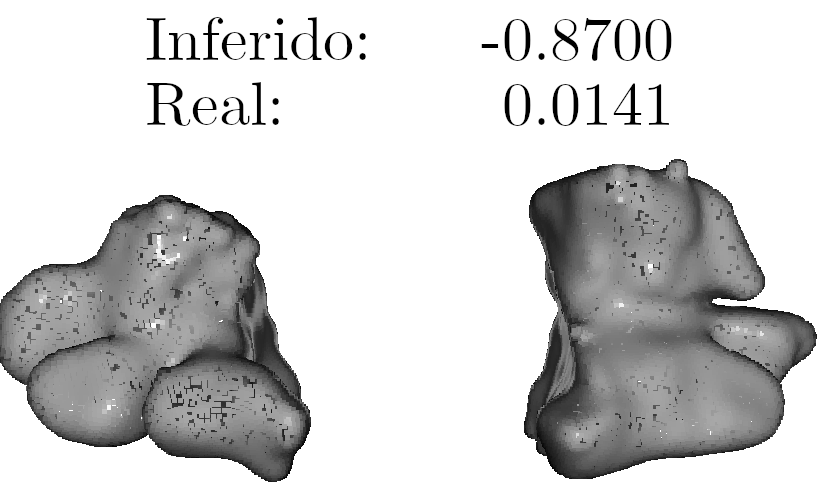
\includegraphics[width=\textwidth]{imagenes/chapter6/Maxiliar100014_7.png}
  \caption{Submuestreo del 10\%.}
\end{subfigure}\hspace{10pt}
  \begin{subfigure}[b]{0.31\textwidth}
  \centering
    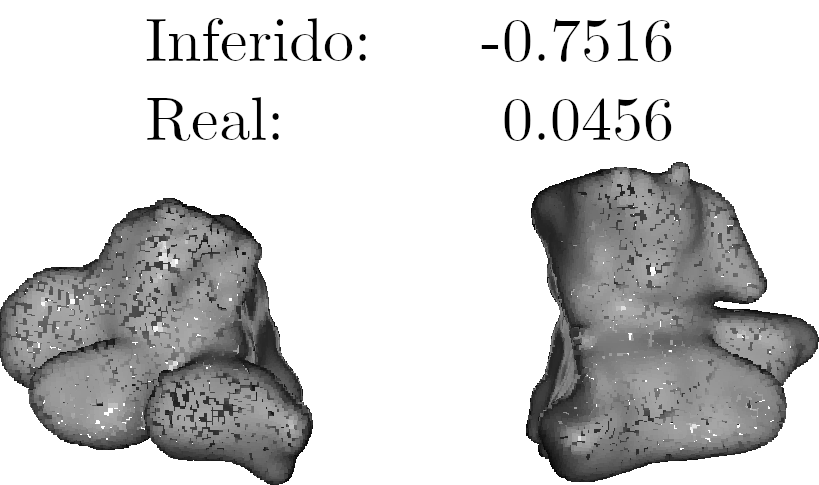
\includegraphics[width=\textwidth]{imagenes/chapter6/Maxiliar100014_9.png}
  \caption{Submuestreo del 30\%.}
\end{subfigure}\hspace{10pt}
  \begin{subfigure}[b]{0.31\textwidth}
  \centering
    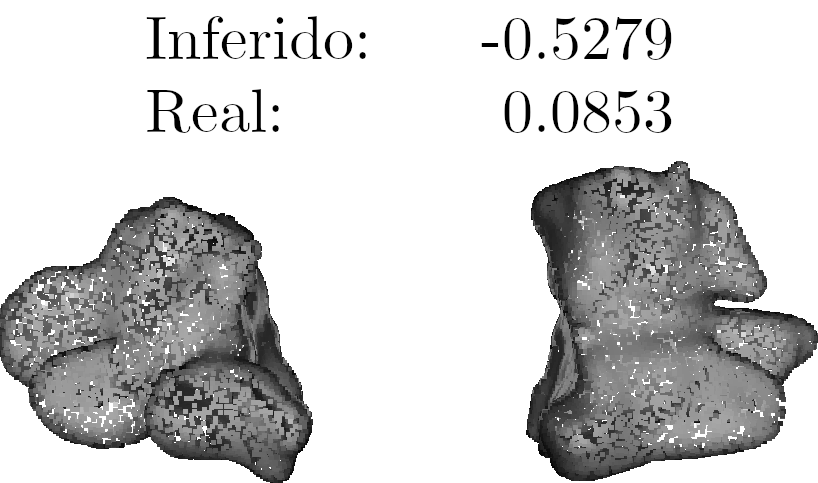
\includegraphics[width=\textwidth]{imagenes/chapter6/Maxiliar100014_11.png}
  \caption{Submuestreo del 60\%.}
  \end{subfigure}
  \caption{Ejemplo de correspondencia de pendiente entre valores inferidos (sin normalizar) y 
  los valores reales de las etiquetas.} 
  \label{fig:Cualitativos}
\end{figure}


Siendo un proyecto en una nueva línea de investigación, existen varias ampliaciones 
lógicas que se pueden realizar a este proyecto. Por un lado, se podría 
obtener una etiqueta manual con un experimento de evaluación, según los estándares, para 
obtener una opinión media de calidad (MOS) y volver a validar los resultados obtenidos
entre los distintos modelos. Así como utilizar ese conjunto de MOS manual sobre imágenes médicas 
para normalizar las etiquetas sintéticas como lo hacen en la publicación original~\cite{ResSCNN}, 
en donde se parte de un conjunto pequeño extraído manualmente para obtener uno sintético varias 
veces más grande. También, para mejorar el método propuesto, se podría permitir 
que los pesos del modelo utilizado para la extracción de características 
del vídeo fueran alterados en vez de ser solamente un paso previo, de extracción. 
De esta forma se podría guiar el modelo a buscar nuevas características temporales.  
Además, se podría buscar simular las distorsiones 
sobre el conjunto de imágenes 2D generadas tras el examen en vez de hacerlo 
sobre la representación 3D final, teniendo así datos más realistas. 

Por otro lado, se pueden explorar otros métodos que procesen modelos 3D directamente, 
o que hagan uso de proyecciones y de la nube de puntos simultáneamente, como en MM-PCQA~\cite{MM-PCQA}.
Actualmente, ha crecido el número de publicaciones de adaptaciones de PointNet~\cite{PointNet} y 
PointNet++~\cite{PointNet++} para resolver distintos problemas de nubes de puntos, 
por lo que quizás se podría adaptar para la resolución de este problema, como 
el método de ResSCNN~\cite{ResSCNN} y evitar así 
la pérdida de información al proyectar en 2D.
